\documentclass[tikz,border=10pt]{standalone}
\usepackage[T1]{fontenc}
\usepackage{helvet}
\renewcommand{\familydefault}{\sfdefault}
\usepackage{tikz}
\usetikzlibrary{arrows.meta,positioning,shapes.multipart,shapes.geometric,fit,backgrounds,calc,shadows}

\definecolor{navy}{HTML}{1F3A5F}
\definecolor{teal}{HTML}{0C6B58}
\definecolor{amber}{HTML}{D9822B}
\definecolor{crimson}{HTML}{B42318}
\definecolor{violet}{HTML}{6B21A8}
\definecolor{sky}{HTML}{2186EB}
\definecolor{slate}{HTML}{486581}
\definecolor{mist}{HTML}{F0F4F8}
\definecolor{line}{HTML}{9FB3C8}

\tikzset{
  >={Stealth[length=2.6mm]},
  box/.style={draw=navy, very thick, rounded corners=3pt, fill=white, align=center,
    inner sep=5pt, font=\small, minimum height=9mm},
  softbox/.style={box, draw=slate, thick, fill=mist},
  layer/.style={draw=line, dashed, rounded corners=6pt, inner sep=7pt},
  layertitle/.style={font=\bfseries\small, text=slate, anchor=north west},
  flow/.style={->, thick, draw=navy},
  dflow/.style={->, thick, draw=slate, dashed},
  lbl/.style={font=\scriptsize, text=slate, fill=white, inner sep=1.5pt},
  umlclass/.style={draw=navy, thick, fill=white, rectangle split, rectangle split parts=3,
    rectangle split part fill={navy!12,white,white}, align=left, font=\scriptsize,
    inner sep=3pt, text width=#1},
  umlclass/.default=38mm,
}

\tikzset{
  entity/.style={draw=navy, very thick, fill=white, rectangle split, rectangle split parts=2,
    rectangle split part fill={navy!14,white}, align=left, font=\scriptsize, inner sep=4pt,
    text width=#1},
  entity/.default=44mm,
  rel/.style={thick, draw=navy},
  card/.style={font=\small\bfseries, text=crimson},
  verb/.style={font=\scriptsize\itshape, text=slate, fill=white, inner sep=1.5pt},
}
\newcommand{\pk}[1]{\underline{\textbf{#1}}}
\newcommand{\fk}[1]{\textit{#1}}
\begin{document}
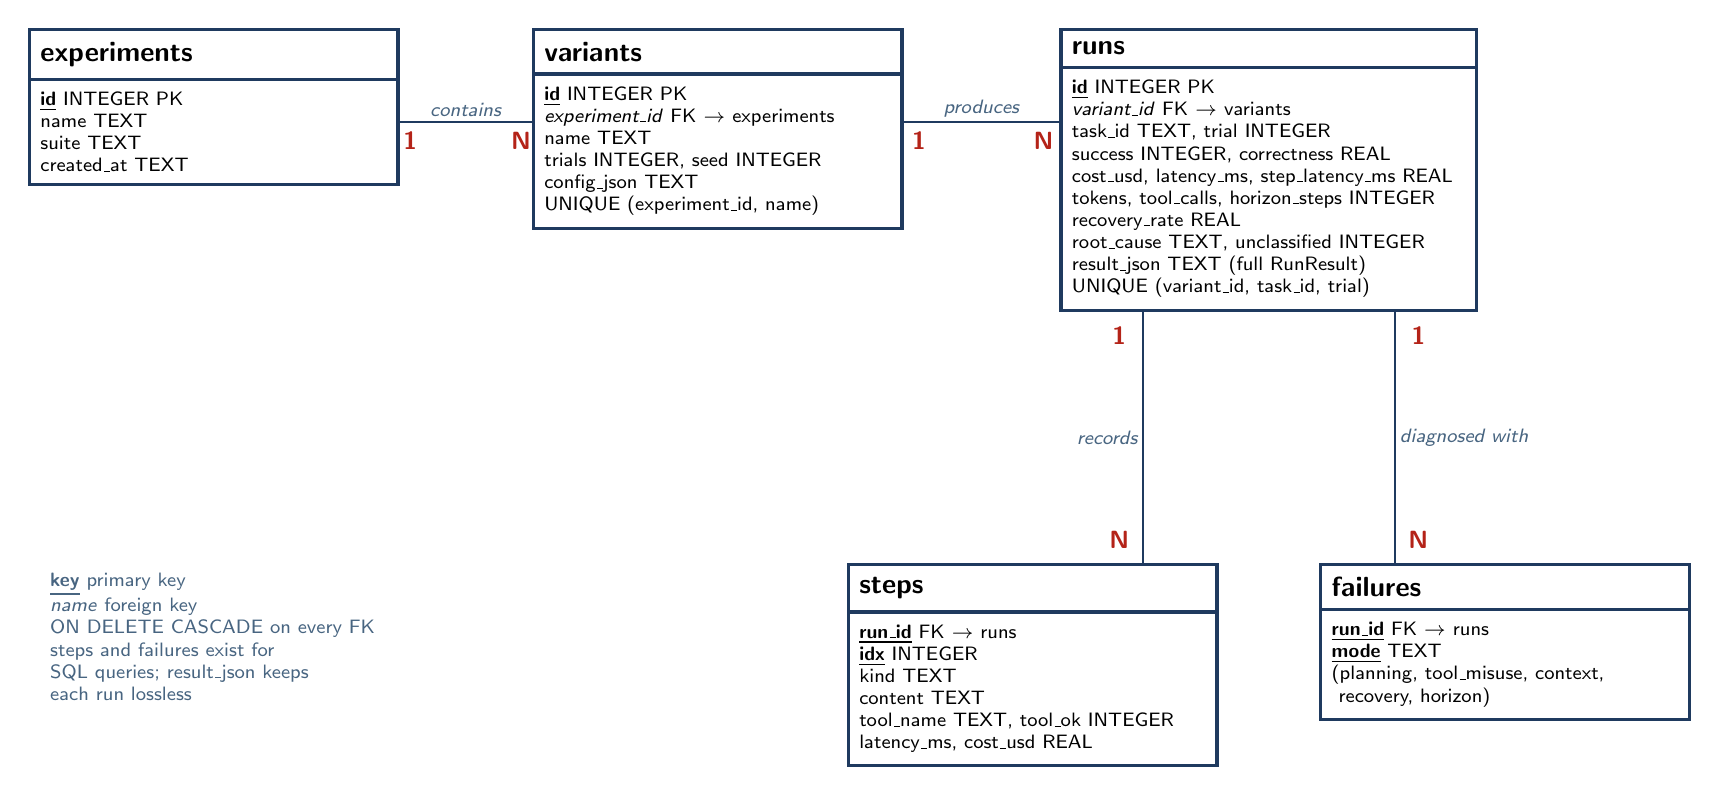
\begin{tikzpicture}[x=1cm,y=1cm]
  \node[entity, anchor=north] (exp) at (0,0) {\textbf{\normalsize experiments}
    \nodepart{second} \pk{id} INTEGER PK\\ name TEXT\\ suite TEXT\\ created\_at TEXT};
  \node[entity, anchor=north] (var) at (6.4,0) {\textbf{\normalsize variants}
    \nodepart{second} \pk{id} INTEGER PK\\ \fk{experiment\_id} FK $\rightarrow$ experiments\\ name TEXT\\ trials INTEGER, seed INTEGER\\ config\_json TEXT\\ UNIQUE (experiment\_id, name)};
  \node[entity=50mm, anchor=north] (run) at (13.4,0) {\textbf{\normalsize runs}
    \nodepart{second} \pk{id} INTEGER PK\\ \fk{variant\_id} FK $\rightarrow$ variants\\ task\_id TEXT, trial INTEGER\\ success INTEGER, correctness REAL\\ cost\_usd, latency\_ms, step\_latency\_ms REAL\\ tokens, tool\_calls, horizon\_steps INTEGER\\ recovery\_rate REAL\\ root\_cause TEXT, unclassified INTEGER\\ result\_json TEXT (full RunResult)\\ UNIQUE (variant\_id, task\_id, trial)};
  \node[entity, anchor=north] (step) at (10.4,-6.8) {\textbf{\normalsize steps}
    \nodepart{second} \pk{\fk{run\_id}} FK $\rightarrow$ runs\\ \pk{idx} INTEGER\\ kind TEXT\\ content TEXT\\ tool\_name TEXT, tool\_ok INTEGER\\ latency\_ms, cost\_usd REAL};
  \node[entity, anchor=north] (fail) at (16.4,-6.8) {\textbf{\normalsize failures}
    \nodepart{second} \pk{\fk{run\_id}} FK $\rightarrow$ runs\\ \pk{mode} TEXT\\ (planning, tool\_misuse, context,\\ \ recovery, horizon)};

  \draw[rel] (exp.east |- 0,-1.2) -- node[verb, above] {contains} (var.west |- 0,-1.2)
    node[card, pos=0.08, below] {1} node[card, pos=0.92, below] {N};
  \draw[rel] (var.east |- 0,-1.2) -- node[verb, above] {produces} (run.west |- 0,-1.2)
    node[card, pos=0.1, below] {1} node[card, pos=0.9, below] {N};
  \draw[rel] ([xshift=-16mm]run.south) -- node[verb, left, pos=0.5] {records} ([xshift=-16mm]run.south |- step.north);
  \node[card] at ([xshift=-19mm, yshift=-3mm]run.south) {1};
  \node[card] at ([xshift=-19mm, yshift=3mm]run.south |- step.north) {N};
  \draw[rel] ([xshift=16mm]run.south) -- node[verb, right, pos=0.5] {diagnosed with} ([xshift=16mm]run.south |- fail.north);
  \node[card] at ([xshift=19mm, yshift=-3mm]run.south) {1};
  \node[card] at ([xshift=19mm, yshift=3mm]run.south |- fail.north) {N};

  \node[font=\scriptsize, text=slate, align=left, anchor=north west] at (-2.2,-6.8) {\pk{key} primary key\\ \fk{name} foreign key\\ ON DELETE CASCADE on every FK\\ steps and failures exist for\\ SQL queries; result\_json keeps\\ each run lossless};
\end{tikzpicture}
\end{document}
